\documentclass[]{article}
\usepackage{lmodern}
\usepackage{amssymb,amsmath}
\usepackage{ifxetex,ifluatex}
\usepackage{fixltx2e} % provides \textsubscript
\ifnum 0\ifxetex 1\fi\ifluatex 1\fi=0 % if pdftex
  \usepackage[T1]{fontenc}
  \usepackage[utf8]{inputenc}
\else % if luatex or xelatex
  \ifxetex
    \usepackage{mathspec}
    \usepackage{xltxtra,xunicode}
  \else
    \usepackage{fontspec}
  \fi
  \defaultfontfeatures{Mapping=tex-text,Scale=MatchLowercase}
  \newcommand{\euro}{€}
\fi
% use upquote if available, for straight quotes in verbatim environments
\IfFileExists{upquote.sty}{\usepackage{upquote}}{}
% use microtype if available
\IfFileExists{microtype.sty}{%
\usepackage{microtype}
\UseMicrotypeSet[protrusion]{basicmath} % disable protrusion for tt fonts
}{}
\usepackage{graphicx}
\makeatletter
\def\maxwidth{\ifdim\Gin@nat@width>\linewidth\linewidth\else\Gin@nat@width\fi}
\def\maxheight{\ifdim\Gin@nat@height>\textheight\textheight\else\Gin@nat@height\fi}
\makeatother
% Scale images if necessary, so that they will not overflow the page
% margins by default, and it is still possible to overwrite the defaults
% using explicit options in \includegraphics[width, height, ...]{}
\setkeys{Gin}{width=\maxwidth,height=\maxheight,keepaspectratio}
\ifxetex
  \usepackage[setpagesize=false, % page size defined by xetex
              unicode=false, % unicode breaks when used with xetex
              xetex]{hyperref}
\else
  \usepackage[unicode=true]{hyperref}
\fi
\hypersetup{breaklinks=true,
            bookmarks=true,
            pdfauthor={},
            pdftitle={},
            colorlinks=true,
            citecolor=blue,
            urlcolor=blue,
            linkcolor=magenta,
            pdfborder={0 0 0}}
\urlstyle{same}  % don't use monospace font for urls
\setlength{\parindent}{0pt}
\setlength{\parskip}{6pt plus 2pt minus 1pt}
\setlength{\emergencystretch}{3em}  % prevent overfull lines
\setcounter{secnumdepth}{0}

\date{}

\begin{document}

\section{Optical Snail Heart Rate
Monitor}\label{optical-snail-heart-rate-monitor}

\textbf{Quentin Geissmann}

Monitoring physiological variables is crucial in many areas of biology.
It is particularly difficult to study the physiology of small animals
whilst minimising experimental interference or under natural conditions.

Land snails are remarkable for their ability to enter in dormancy states
when the weather becomes too cold (hibernation) or too dry (estivation).
They can remain several months in these respective states as their
metabolism dramatically slows down, which reduces their need for food
and water.

Recording heart rate of snails could reveal a valuable tool to shed
light on the mechanisms underlying these exceptional phenomena. In
addition, it could help to understand temporal patterns of activity and,
for instance, foraging and mating strategies.

Garden snails (\emph{Helix aspersa}) are fairly large terrestrial
invertebrates (more than 10 g for adults) capable of pulling their own
weight several times. In addition, their shell is a stable mineral
support where small circuits can simply be glued with, presumably,
little inconvenience for the animal. It is possible to observe the heart
of young snails, through their thin shell with naked eyes. In adult
snails, the same observation can be achieved by casting strong light
through the shell. It should therefore be possible to measure light
attenuation over time in order to infer heart rate.

For these reasons, land snails appear particularly suited to carrying
small electronic equipment in order to record an important physiological
variable for extended periods of time. This project describes an
inexpensive and non-invasive device to monitor heart rate in land
snails.

\subsection{Project Aim}\label{project-aim}

The aim of this project is to build a small device that can monitor a
snail's heart rate and is small enough to be carried by a garden snail
(\emph{Helix aspersa}). When sending red light though the bottom of the
shell, the moving heart of the snail can be seen. From this observation,
the goal is to fit a low power red LED on one side of the shell whilst
recording the intensity of the transmitted light, using a
phototransistor (PT), from the other side.

In order to keep the device lightweight, thin wires will be used to
convey analogue signal between the animal and an Arduino Uno board.
Then, the serial port will be used to communicate data to a computer
which will display the signal in real time using a \texttt{python}
script.

In order to save energy and reduce the amount of heat generated by the
LED, the circuit will be powered only shortly before recording data
points, and turned off immediately after. For this purpose, a digital
pin will be used.

\subsection{Techniques Used}\label{techniques-used}

\begin{itemize}
\itemsep1pt\parskip0pt\parsep0pt
\item
  Reading values from a PT
\item
  Using a digital pin to drive power
\item
  Oversampling signal to improve resolution of A/D conversion.
\item
  Real time data visualisation using \texttt{python} in combination with
  \texttt{pyserial} and \texttt{pygame}
\end{itemize}

\subsection{Materials}\label{materials}

\begin{itemize}
\itemsep1pt\parskip0pt\parsep0pt
\item
  Arduino Uno
\item
  Computer
\item
  Low voltage (around 3 V) bright red LED. Ideally, a small, surface
  mounted, one with a flat lens and a wide (\textgreater{}100°) angle.
\item
  Phototransistor (PT) that matches the wavelength of the above LED.
\item
  68 Ω resistor
\item
  100 kΩ resistor
\item
  A two rows, straight, PCB header
\item
  A one row PCB socket
\item
  Some thin wire
\item
  Large garden snail
\item
  Superglue
\item
  Blu tack
\item
  A large snail (an adult \emph{Helix aspersa} should be perfect)
\end{itemize}

\textbf{@edwbaker -\textgreater{} you will probably want to change the
links to your cloned/reorganised version here}

\textbf{@edwbaker -\textgreater{} Maybe you want this as a footnote, or
not at all.}

\emph{The commercial references to some of the electronic components can
be found at
(https://github.com/gilestrolab/snail\_back\_pack/blob/master/protocols/rs\_numbers.md)}

\subsection{Code Download}\label{code-download}

\textbf{@edwbaker -\textgreater{} fix links at some point}

\begin{itemize}
\itemsep1pt\parskip0pt\parsep0pt
\item
  Arduino code
  (https://github.com/gilestrolab/snail\_back\_pack/blob/master/arduino\_prototypes/sparse\_phototransistor/sparse\_phototransistor.ino)
\item
  Python code
  (https://github.com/gilestrolab/snail\_back\_pack/blob/master/scripts/serial\_monitor.py)
\end{itemize}

\subsection{Supporting Materials}\label{supporting-materials}

\begin{itemize}
\itemsep1pt\parskip0pt\parsep0pt
\item
  Video of the protocol (http://dx.doi.org/10.6084/m9.figshare.1294198)
\end{itemize}

\subsection{Theory}\label{theory}

Land snails have a semi-closed circular system where their oxygenated
hemolymph (i.e.~blood) is carried from their lung to their heart in a
pulmonary vein. Then, the heart, which has two cavities (atrium and
ventricle), pumps the blood into the aorta artery. As opposed to a
closed circulatory system (e.g.~in vertebrates), the hemolymph then
mixes with the extracellular fluid before diffusing to the lung.

The heart rates of snails is regulated by oxygen demand and can scale
from more to one beat per second (e.g.~when the animal is active and the
temperature high) to as low as one a minute (e.g.~during hibernation).
Much like in vertebrates, the electrical activity of the heart can be
recorded by electrocardiography (ECG) in order to measure heart rate.
However, this technique is quite invasive (i.e.~holes need to be drilled
in the shell), and technically challenging.

In human, pulse-oximetry can be used to reliably and non-invasively
infer heart rate by comparing red and infrared absorbance. In snail,
since a difference in light absorbance is visible during heart beats, it
should be possible to record these variations using simple electronics.

Light-Emitting Diodes (LEDs) are used in a wide range of applications.
They feature low power consumptions and some of them are capable of
generating a relatively narrow emission spectrum (e.g.~95\% of the
emission within a 100 nm band). In this project, we will power an LED
with a forward current \texttt{I\_F\ =\ 40\ mA}, and a forward voltage
\texttt{V\_F\ =\ 2.6\ V} from a \texttt{V\_B\ =\ 5\ V} board. Therefore,
we need to drop \texttt{V\_R\ =\ V\_B\ -\ V\_F\ =\ 2.4\ V} with a
resistor (in series with the LED).

\textbf{@edwbaker =\textgreater{} maths formatting around here?}

According to Ohm's law, the resistance is \texttt{R\ =\ V\_R/I\_F}. So,
in our case, \texttt{R\ =\ 60\ Ω}, which means we should be able to use
a 68 Ω resistor.

Phototransistors (PTs) are essentially transistors that allow variable
current to pass through as a function of light intensity. As opposed to
PTs, they have a relatively fast response time. In order to record light
intensity, we can record how much current ``leaks'' through the PT. To
do so, we put a resistor in series with the PT and measure the voltage
across it with the analogue pin. The value of the resistance affect the
gain and should depend on the type of PT and the range of light
intensity. In our case, a 100 kΩ resistor should give satisfying
results.

\subsection{The circuit}\label{the-circuit}

The circuit in itself is really simple:

\begin{figure}[htbp]
\centering
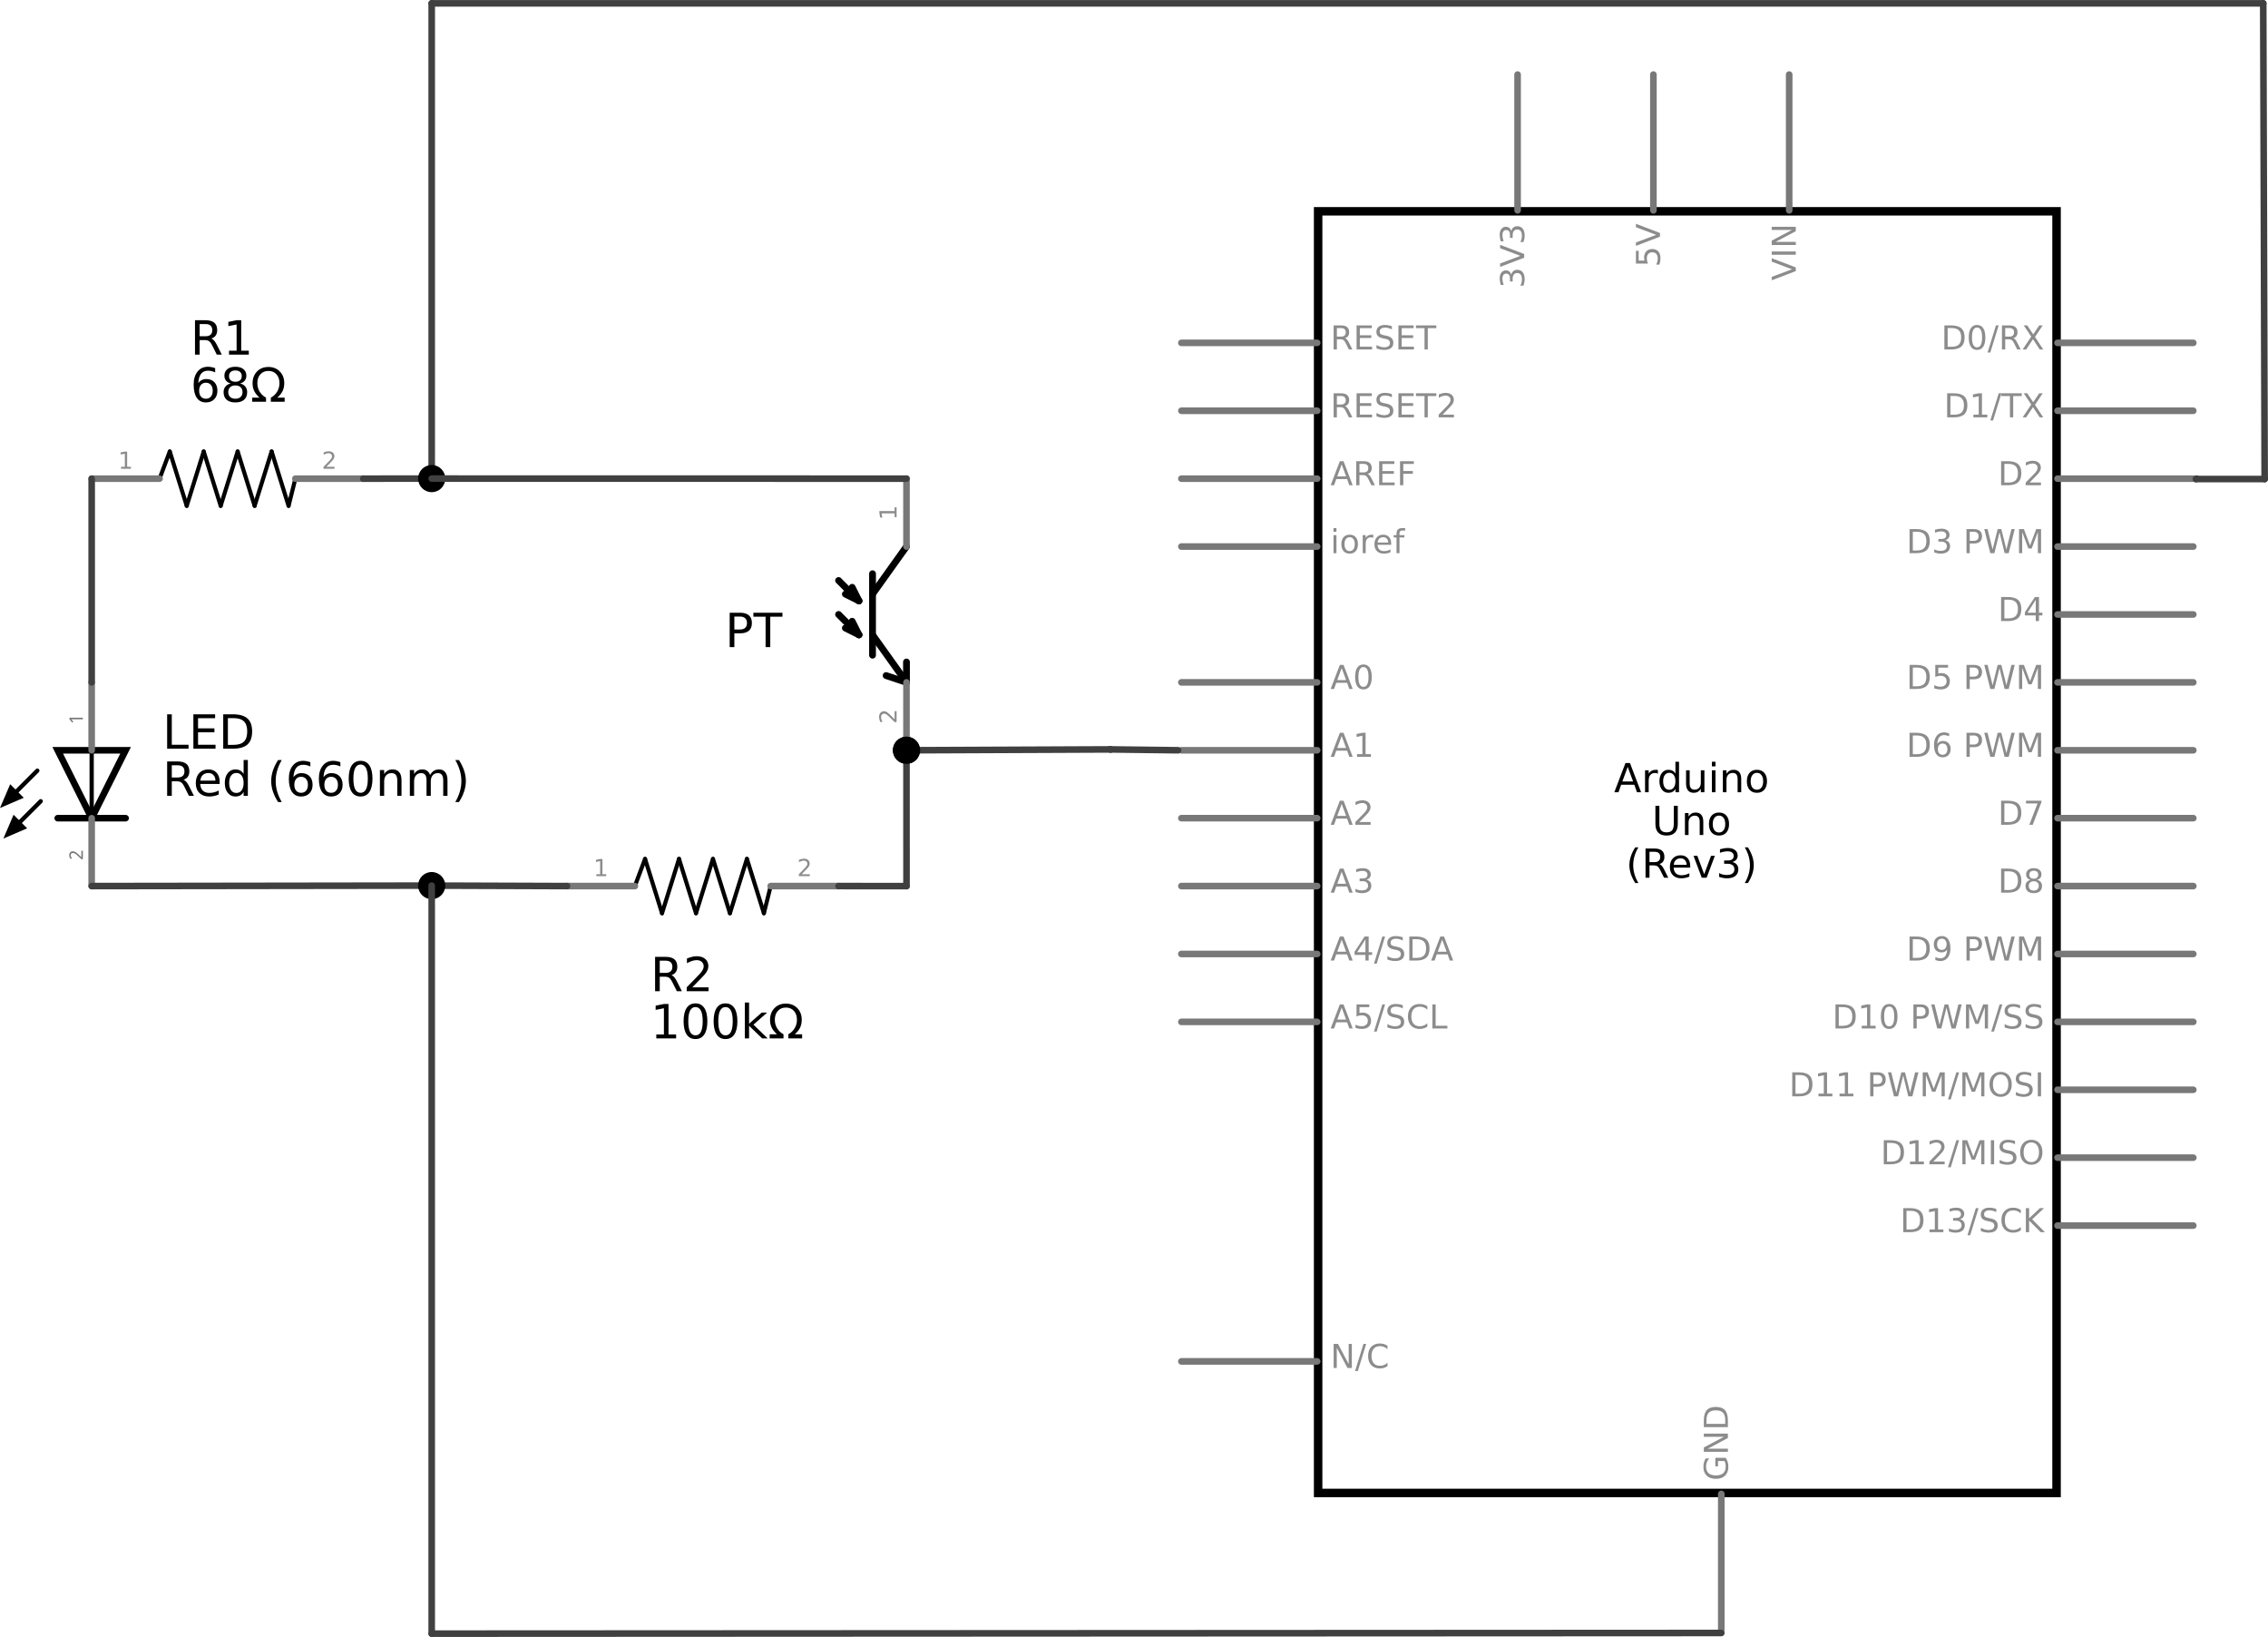
\includegraphics{./img/circuit.png}
\caption{Circuit schematic}
\end{figure}

Note that the \textbf{digital pin 2 is used instead of the 5 V pin}.
This way, we can turn the circuit on and off from the Arduino.

\subsection{Putting it Together}\label{putting-it-together}

The end goal is to build a sort of saddle that can be glued onto the
shell, and then plugged to wires for recording purposes. View from the
bottom, the final product could look like this:

\begin{figure}[htbp]
\centering
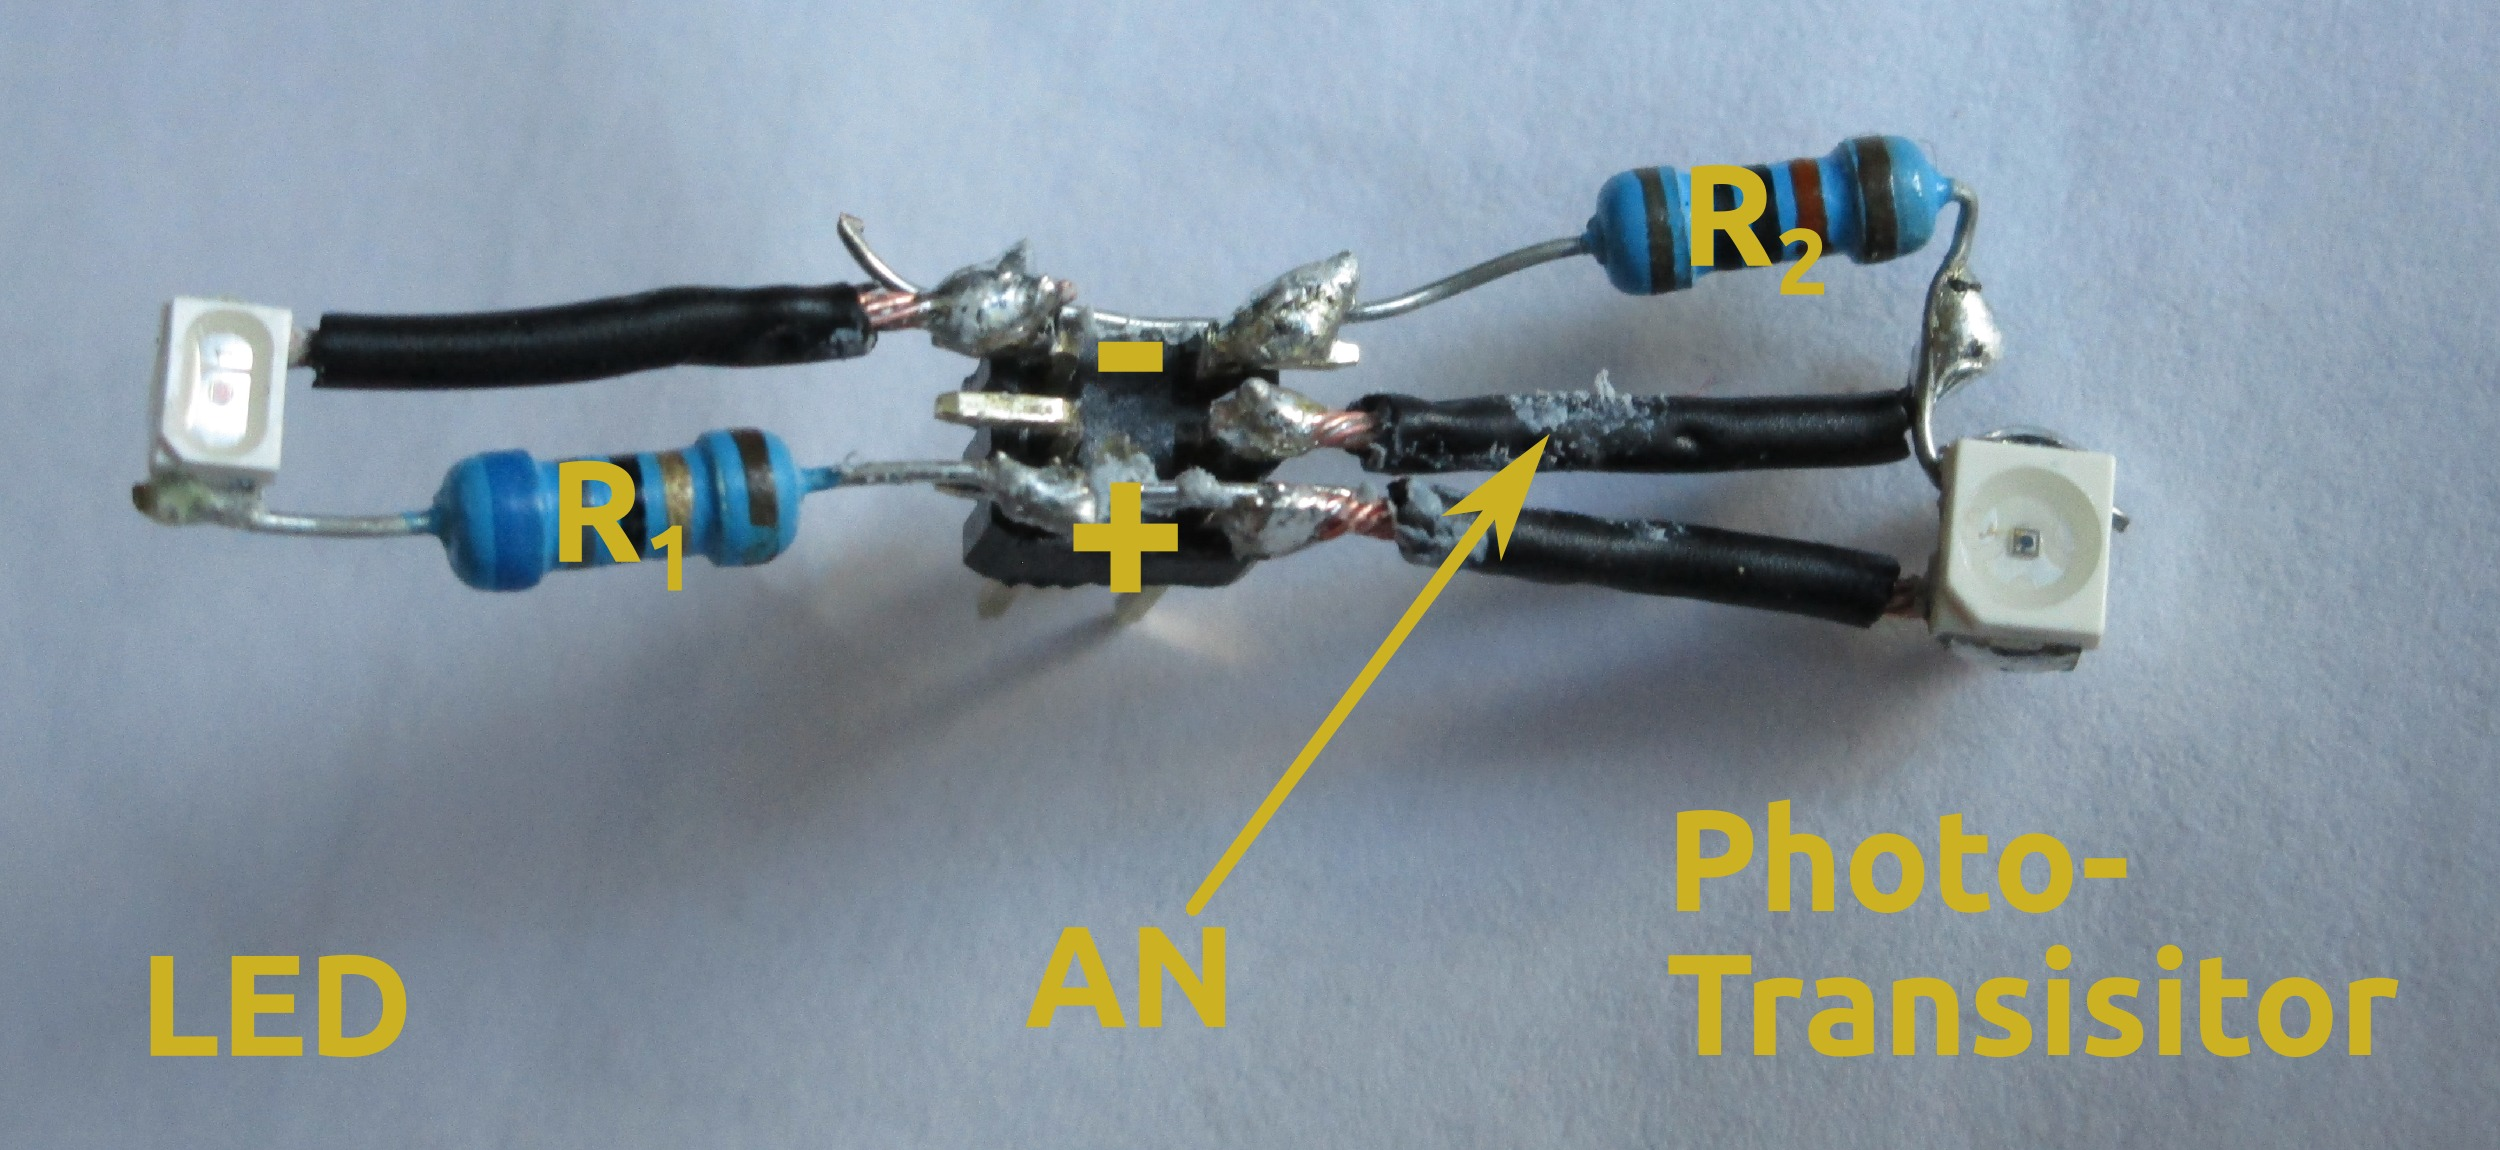
\includegraphics{./img/fig1.jpg}
\caption{Monitoring device, bottom view}
\end{figure}

And from the top:

\begin{figure}[htbp]
\centering
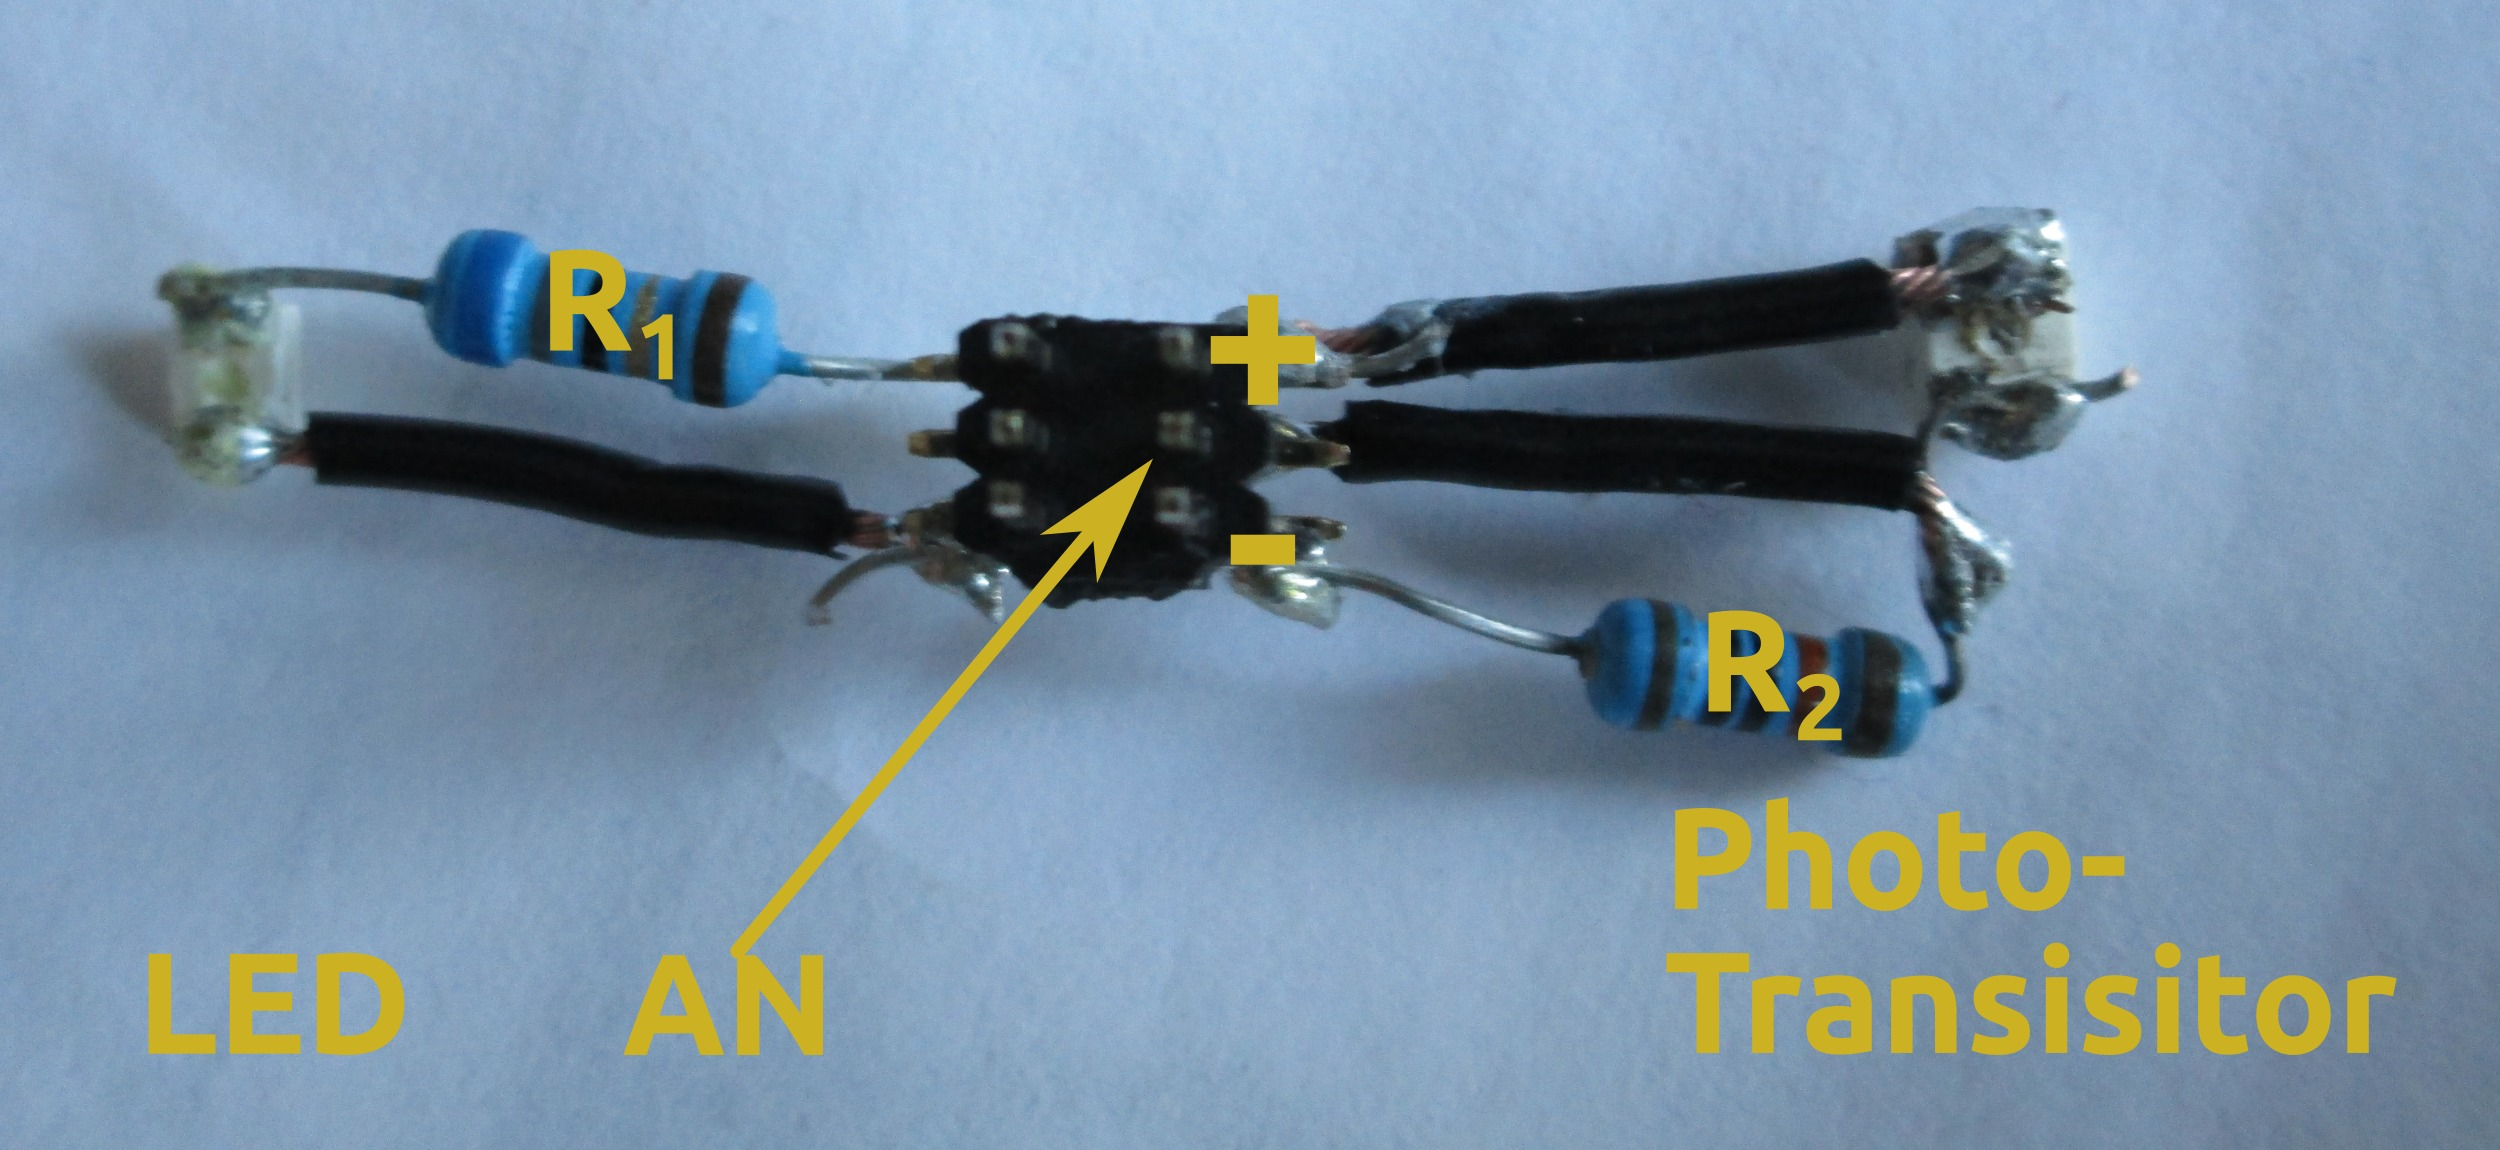
\includegraphics{./img/fig2.jpg}
\caption{Monitoring device, top view}
\end{figure}

In both figures, `\texttt{AN}' is for the analogue pin.

\subsection{General Instructions}\label{general-instructions}

We will use the leads of the resistors, and some wire, as a skeleton for
our device. Therefore, we will wait until the end to cut them. Soldering
the LED and the PT can reveal challenging as both parts are very small.
So, it is recommended to hold them firmly, for instance, using ``helping
hands''. It is easy to forget that both \textbf{LED and PT should face
downward} as the light will be transmitted through the shell.

\subsection{The LED}\label{the-led}

\begin{enumerate}
\def\labelenumi{\arabic{enumi}.}
\itemsep1pt\parskip0pt\parsep0pt
\item
  Before starting, ensure you can tell cathode and anode apart. Most
  ``surface mounted LEDs'' will have an indication such as a small chip
  on the \texttt{+} side.
\item
  Solder directly one lead of the 68 Ω resistor to the anode of the LED.
\item
  Cut a short wire (1 cm). Strip and twist its tip.
\item
  Solder one extremity of the wire to the cathode.
\end{enumerate}

\subsection{The Phototransistor (PT)}\label{the-phototransistor-pt}

\begin{enumerate}
\def\labelenumi{\arabic{enumi}.}
\itemsep1pt\parskip0pt\parsep0pt
\item
  As for the LED, ensure you know the polarity.
\item
  Cut two short wires (1 cm). Strip and twist their tips.
\item
  Solder one extremity of a wire to the anode of the PT.
\item
  Solder directly one lead of the 100 kΩ resistor to the cathode. Leave
  some space between the anode and the resistor to solder the second
  wire.
\item
  Solder the tip of the second wire onto the lead of the resistor;
  between the resistor and the PT.
\end{enumerate}

\subsection{Assembling on the PCB
header}\label{assembling-on-the-pcb-header}

\begin{enumerate}
\def\labelenumi{\arabic{enumi}.}
\itemsep1pt\parskip0pt\parsep0pt
\item
  Cut the PCB headed to leave only three columns (i.e.~6pins). From a
  bottom-up view, let us label the pins:
\end{enumerate}

\begin{figure}[htbp]
\centering

\includegraphics{./img/header_map.png}
\caption{PCB header map}
\end{figure}

\begin{enumerate}
\def\labelenumi{\arabic{enumi}.}
\setcounter{enumi}{1}
\itemsep1pt\parskip0pt\parsep0pt
\item
  Solder the wire connected to the LED light on A. That is on the
  \texttt{-} side.
\item
  Solder the lead of the resistor connected to the LED on C \textbf{and
  F} (i.e. \texttt{+} side).
\item
  Solder the wire connected the anode of the PT to F.
\item
  Solder the leg of the resistor connected to the PT on A \textbf{and
  D}.
\item
  Solder the second wire of the PT on E.
\end{enumerate}

\subsection{Lead}\label{lead}

\begin{enumerate}
\def\labelenumi{\arabic{enumi}.}
\itemsep1pt\parskip0pt\parsep0pt
\item
  Strip the tips of three long (\textgreater{}30cm) flexible and thin
  wires.
\item
  Cut three columns of the PCB socket.
\item
  Solder each wire to a different pin of the PCB header.
\item
  Plug the PCB socket on the pins \texttt{D}, \texttt{E} and \texttt{F}
  of the PCB header.
\item
  Unsure you can tell which wire is for ground (pin \texttt{D}), and
  which is for \texttt{+} (pin \texttt{F}).
\end{enumerate}

\subsection{Arduino}\label{arduino}

\begin{enumerate}
\def\labelenumi{\arabic{enumi}.}
\itemsep1pt\parskip0pt\parsep0pt
\item
  Plug the \texttt{+} wire on digital pin 2 -- or 5 V if you want
  constant light (see `Fitting the Circuit' section below).
\item
  Plug the ground wire on ground.
\item
  Plug the middle wire on analogue in 1.
\item
  Compile and upload the code for this project to the Arduino.
\item
  The LED light should start blinking quickly.
\end{enumerate}

\subsection{Fitting the Circuit}\label{fitting-the-circuit}

This is probably the hardest part of the process. For this reason, a
four minutes video demonstrating this part of the protocol step by step
is available online (see `Supporting Material' section above).

The main steps are:

\begin{enumerate}
\def\labelenumi{\arabic{enumi}.}
\itemsep1pt\parskip0pt\parsep0pt
\item
  Protect the animal by putting tissue paper on the opening of the
  shell.
\item
  Plug the Arduino to the USB port of your computer.
\item
  Run the \texttt{python} program (see `Code Download' section above). A
  window should appear and plot the signal in real time (see section
  `Python Code Complementary' below).
\item
  Plug the circuit on. For now, \emph{use the 5 V pin} instead of the
  digital pin as it will allow you to see the heart beating much better.
\item
  At this stage, you should be able to test the circuit by moving
  objects between PT and LED, and observe variation in the data
  displayed by the \texttt{python} program.
\item
  Move the LED on the shell until you see the beating heart with your
  eyes.
\item
  Use blu tack to maintain the circuit on the shell, and assess the
  quality of the signal displayed on your screen.
\item
  Move the PT until the signal to noise ratio is satisfying (i.e.~sharp
  oscillations of large amplitude). Then glue PT and LED to the shell.
\item
  Unplug the circuit, interrupt the \texttt{python} program, and wait
  for the glue to dry.
\item
  Plug the circuit. This time, \textbf{use the analogue pin} as opposed
  to the 5 V.
\item
  Run the \texttt{python} program. In addition to simply display heart
  rate, the data can be saved to a text file using the \texttt{-\/-out}
  option (see section `Python Code Complementary' below).
\end{enumerate}

In the end, the animal should have no difficulty to move with the
device:

\begin{figure}[htbp]
\centering
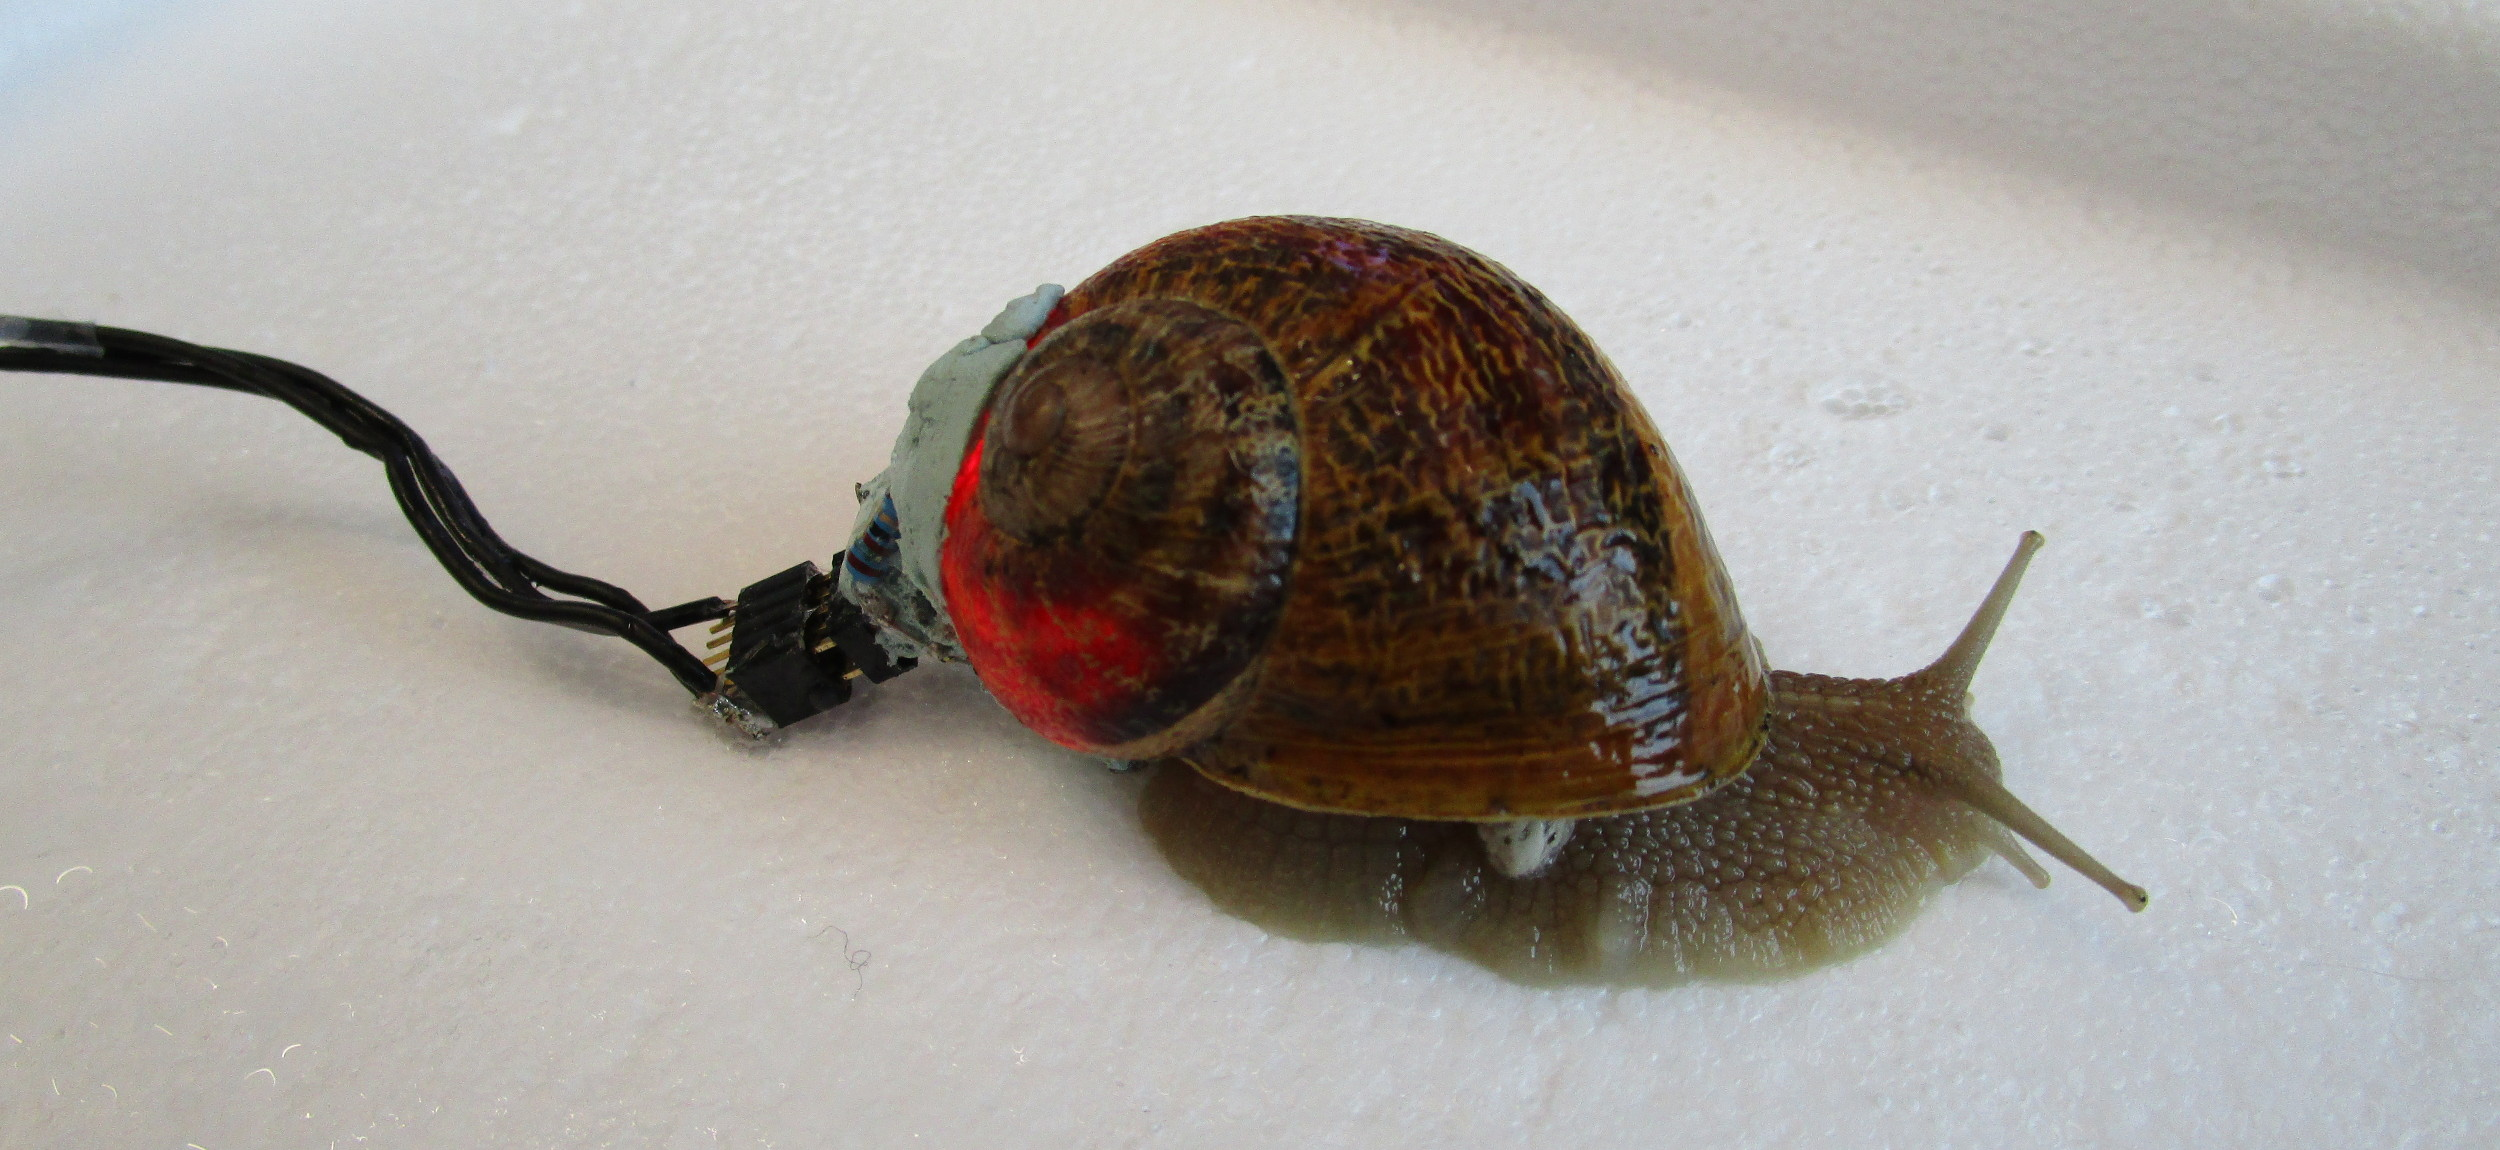
\includegraphics{./img/snail_with_device.jpg}
\caption{Snail with device}
\end{figure}

\textbf{Important Note:}

\begin{itemize}
\itemsep1pt\parskip0pt\parsep0pt
\item
  Use as little glue as possible and \textbf{do not} touch the foot of
  the animal with any glue. If you are concerns about the toxicity of
  the glue, you may consider alternatives such as dental cement.
\end{itemize}

\subsection{Arduino Code
Complementary}\label{arduino-code-complementary}

This project only contains a short file. We start by defining numerical
constants:

\begin{verbatim}
#define OVER_SAMPLING 16
#define FS 5.0 // in Hz
#define RISE_TIME 1 // in ms
#define POWER_PIN 2
#define PHOTO_TRANSISTOR_PIN 1
\end{verbatim}

\begin{itemize}
\itemsep1pt\parskip0pt\parsep0pt
\item
  Every data point will be the sum of \texttt{OVER\_SAMPLING}
  consecutive reads.
\item
  The sampling frequency \texttt{FS} (in Hz). That is the actual number
  of point we output every second.
\item
  \texttt{RISE\_TIME} defines how long should we leave the circuit
  turned on before reading any value.
\item
  The digital pin controlling power is number 2.
\item
  The analogue pin from which PT values are read is number 1.
\end{itemize}

Then, we compute the time to wait between consecutive reads:

\begin{verbatim}
const float time_to_sleep_ms = 1e3/(FS*OVER_SAMPLING) - RISE_TIME;
\end{verbatim}

Since are performing \emph{oversampling} every data point we output is,
in fact, the sum of several (in this example, exactly 16) reads.
Therefore, the actual reading sampling frequency
\texttt{Fs\_a\ =\ Fs\ *\ s} where \texttt{Fs} is the resulting sampling
frequency (i.e.~5 Hz) and \texttt{s}, the oversampling factor (i.e.~16
times). The delay \texttt{dt} between two actual reads is then simply
\texttt{1/Fs\_a} (in seconds).

Note that we also subtract the rise time to be more accurate. Also, we
multiply by 1000 since we want milliseconds instead of seconds.

In the setup:

\begin{verbatim}
void setup(void) {
    Serial.begin(57600);
    pinMode(POWER_PIN, OUTPUT);
}
\end{verbatim}

We simply:

\begin{itemize}
\itemsep1pt\parskip0pt\parsep0pt
\item
  Set the baud rate to 57600, which should be more than enough.
\item
  Set the digital pin as an output pin that can take HIGH(5 V) or LOW(0
  V) values.
\end{itemize}

And in the main loop:

\begin{verbatim}
void loop(void) {
    unsigned int accum = 0;
    for(int i =0; i < OVER_SAMPLING; i++){
        digitalWrite(POWER_PIN, HIGH);
        delay(RISE_TIME);
        accum +=  analogRead(PHOTO_TRANSISTOR_PIN);
        digitalWrite(POWER_PIN, LOW);
        delay(time_to_sleep_ms) ;
    }
    Serial.println(accum);
}
\end{verbatim}

For each iteration:

\begin{enumerate}
\def\labelenumi{\arabic{enumi}.}
\itemsep1pt\parskip0pt\parsep0pt
\item
  We initialise an accumulator variable to 0.
\item
  We are going to sample as many time as the value of
  \texttt{OVER\_SAMPLING}, so we start a for loop in which we:

  \begin{enumerate}
  \def\labelenumii{\arabic{enumii}.}
  \itemsep1pt\parskip0pt\parsep0pt
  \item
    Turn the circuit ON.
  \item
    Wait for the circuit to be in a stationary state.
  \item
    Read the PT value.
  \item
    We increment the accumulator by the obtain value.
  \item
    We immediately turn the circuit OFF.
  \item
    We sleep for the delay \texttt{dt}.
  \end{enumerate}
\item
  When the above loop completes, we can send the value of the
  accumulator to the serial port in order to use it from a connected
  computer.
\end{enumerate}

\subsection{Python Code Complementary}\label{python-code-complementary}

This project uses \texttt{python} programing language for real time
visualisation on a computer screen. Importantly, \texttt{python2} (not
\texttt{python3}) should be run.

\begin{enumerate}
\def\labelenumi{\arabic{enumi}.}
\item
  Install \texttt{python2} on your machine.
\item
  Install dependency packages using. You can use \texttt{pip}, the
  python package manager for that:

\begin{verbatim}
pip install numpy pyserial
\end{verbatim}
\item
  Install \texttt{pygame} (http://pygame.org/download.shtml).
  \textbf{@edwbaker -\textgreater{} I am not sure how/if you want to
  display urls inline}
\item
  Download the \texttt{python} code (see `Code Download' section above)
\item
  Open a terminal and run the \texttt{python} code. For instance:

\begin{verbatim}
python serial_monitor.py --port /dev/ttyACM0
\end{verbatim}

  Note that you may need to set a different serial port (e.g.
  \texttt{-\/-port\ /MY/PORT/IS/HERE}) according to your machine and
  operating system. In addition, other options can be displayed by:

  \texttt{python\ serial\_monitor.py\ -\/-help}

  For instance, \texttt{-\/-out\ /WHERE/TO/SAVE/THE/data.txt} can be
  useful.
\end{enumerate}

When running the program, a visualisation window should appear:

\begin{figure}[htbp]
\centering
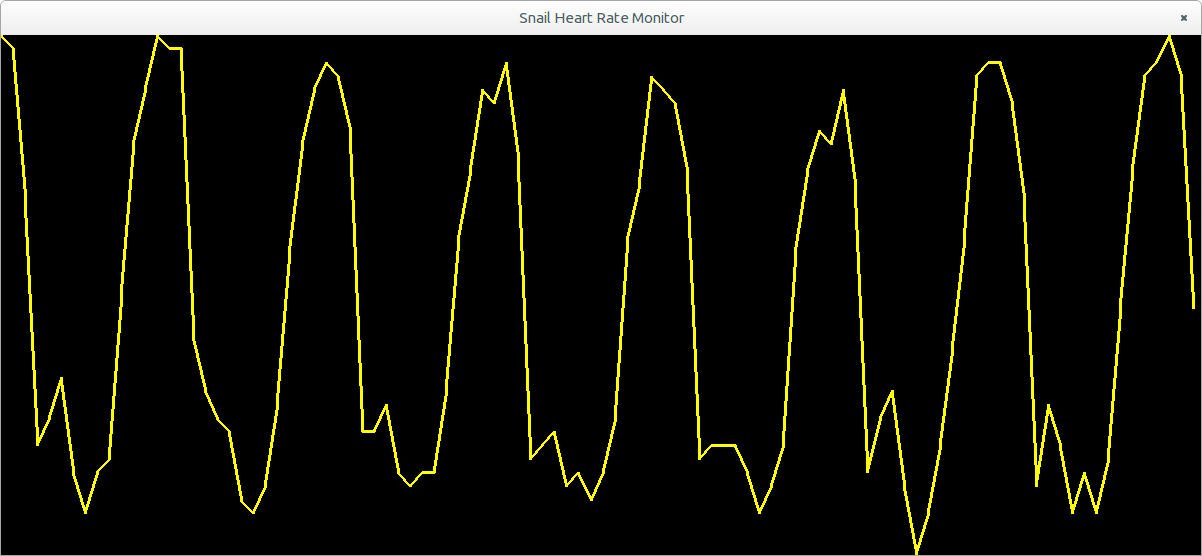
\includegraphics{./img/python_window.png}
\caption{Real time visualisation window}
\end{figure}

If you are interested in understanding or adapting this python script,
explanations are provided, as comments, within the source code.

\subsection{Example of Result}\label{example-of-result}

This is an example of approximately one minute of real data, sampled at
10 Hz:

\begin{figure}[htbp]
\centering
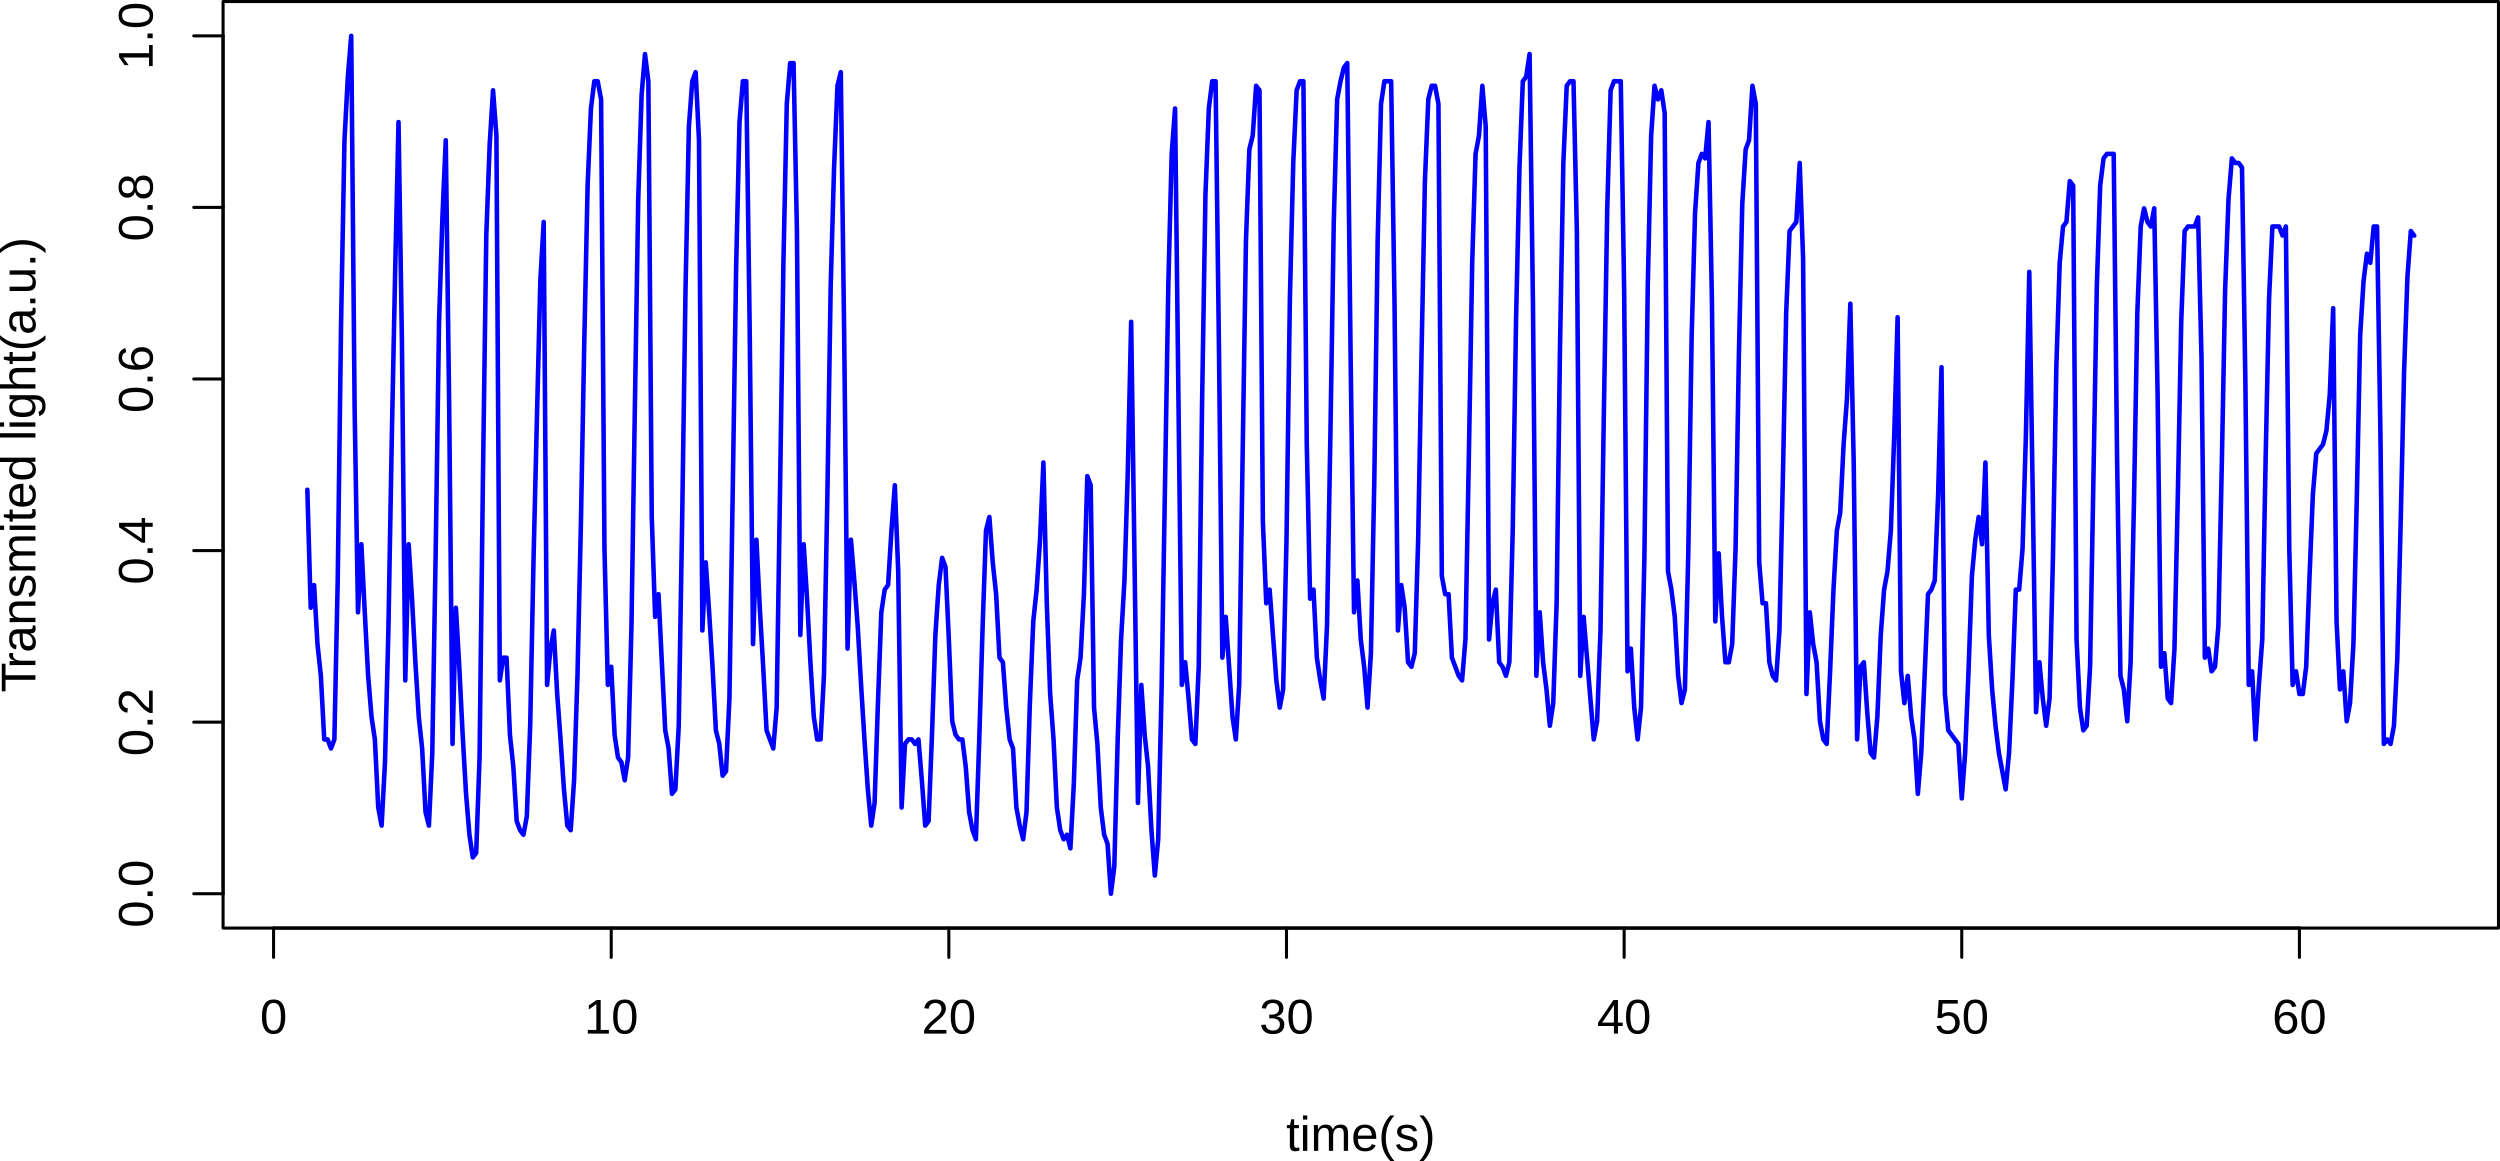
\includegraphics{./img/one_min_data.png}
\caption{One minute of data}
\end{figure}

The corresponding power spectrum indicates a fundamental frequency
around 0.75 Hz (vertical dashed line), which is 45 beats per minute:

\begin{figure}[htbp]
\centering
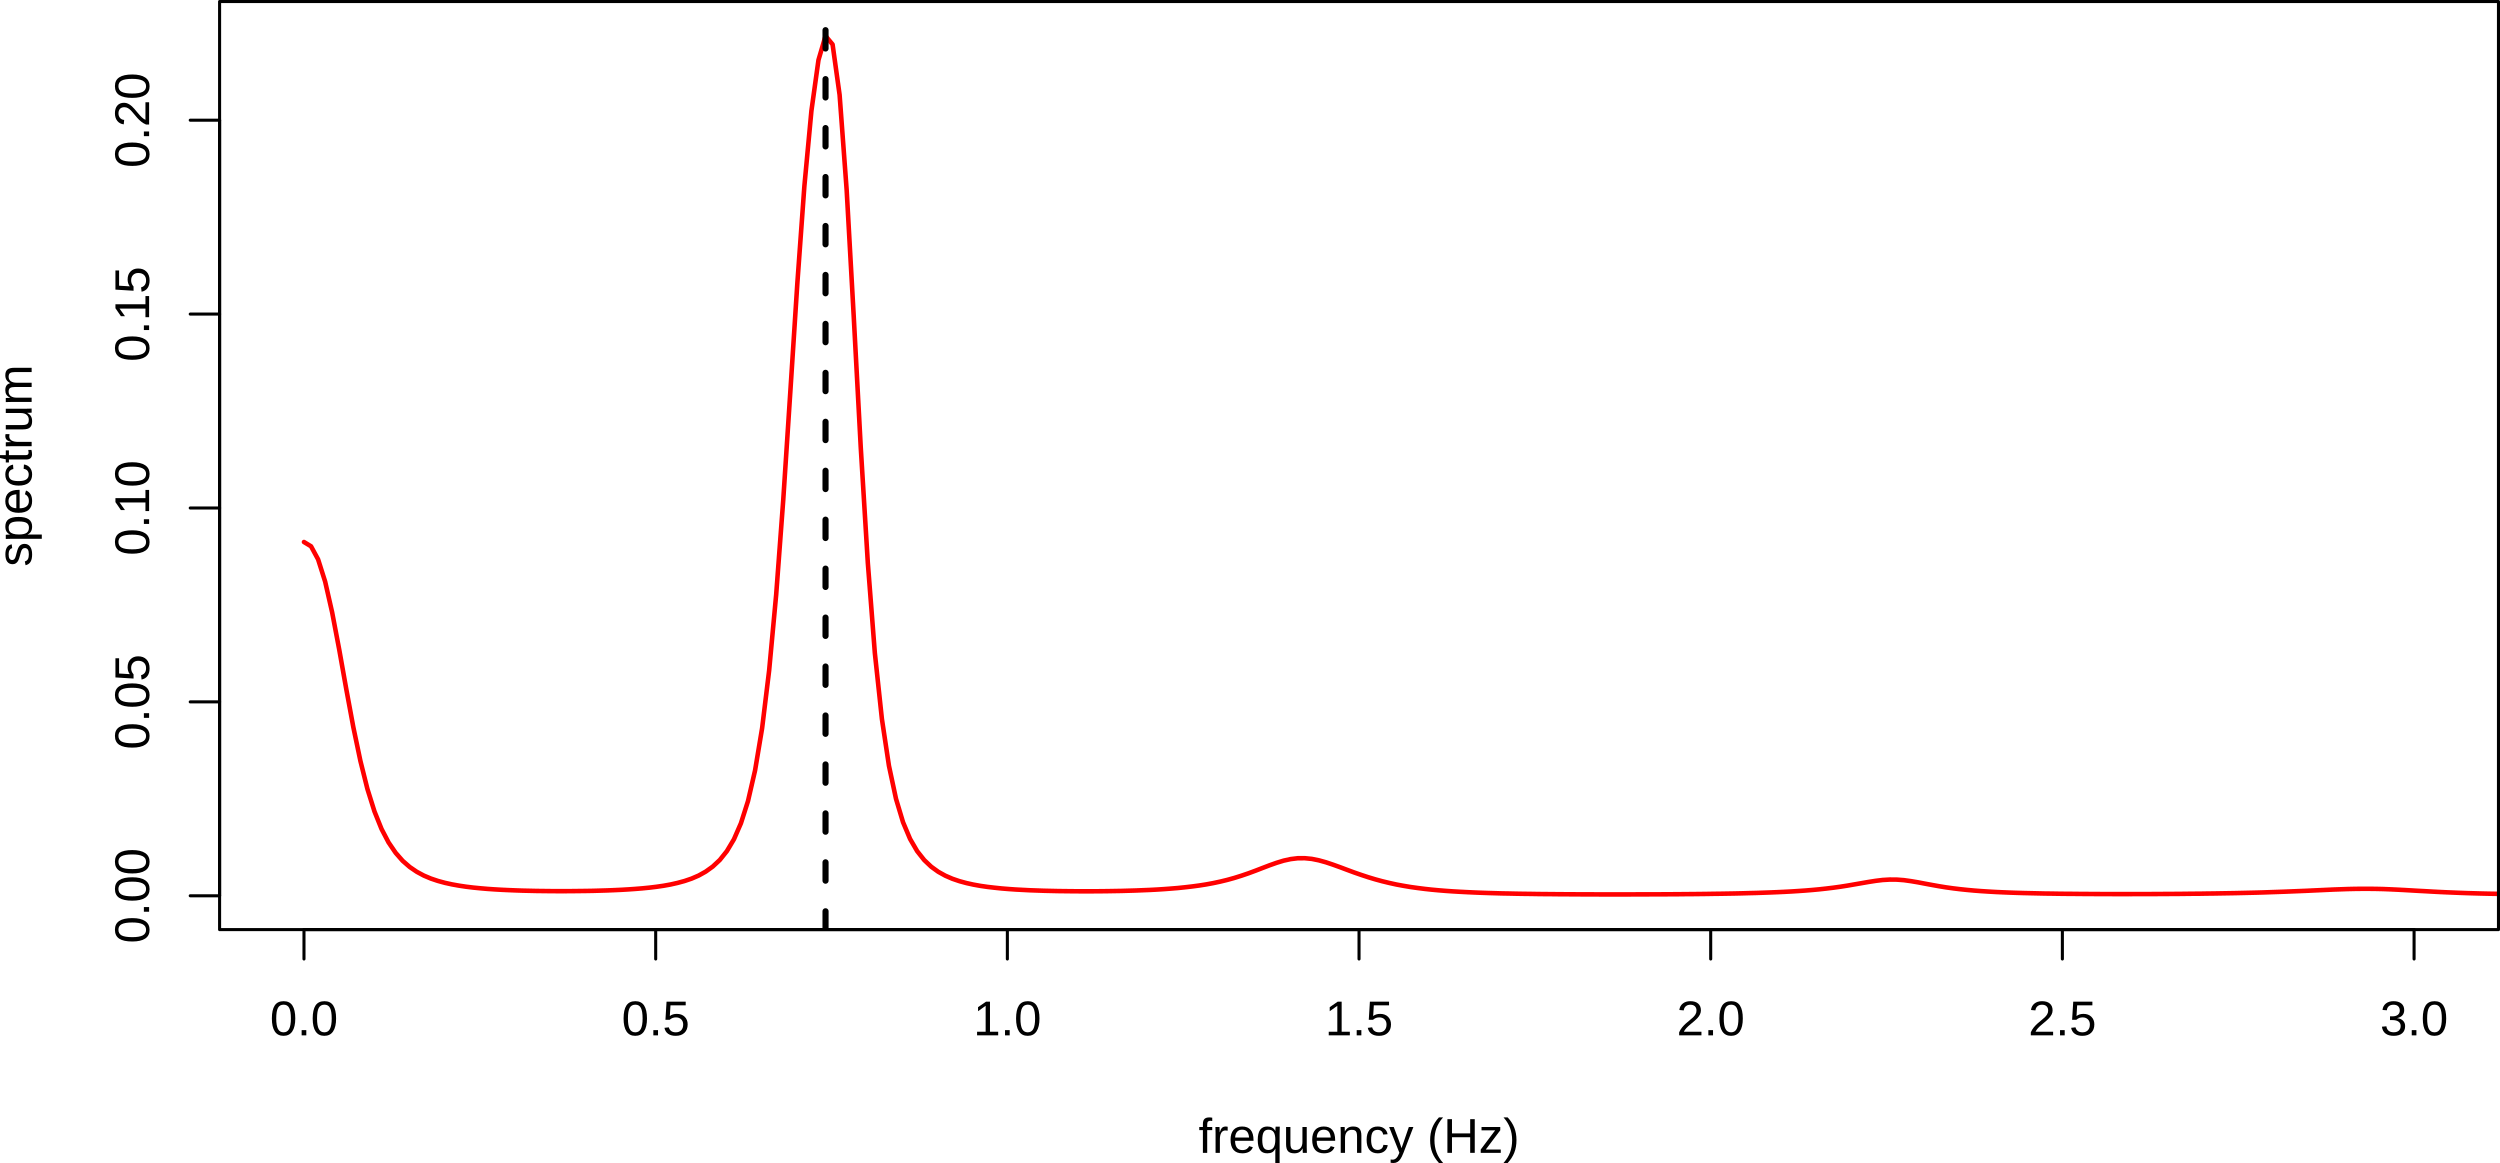
\includegraphics{./img/power_spectrum.png}
\caption{Power spectrum}
\end{figure}

\subsection{Next steps}\label{next-steps}

Improvements to this method are currently under investigation and
include:

\begin{itemize}
\itemsep1pt\parskip0pt\parsep0pt
\item
  Using infrared instead of red light in order to reduce environmental
  noise.
\item
  Computing heart rate directly on the Arduino board.
\item
  Developing a wireless version.
\item
  Using several PTs to increase accuracy and robustness.
\end{itemize}

\end{document}
